% fig18-followup-basins.tex
% Matched deep-basin subset in the paper cohort
\documentclass[tikz,border=18pt]{standalone}
% common-styles.tex
% Shared TikZ styles for wonton-proof paper figures

\usepackage{silence}
\WarningFilter{latex}{Missing character} 
\tracinglostchars=0 % Suppress engine-level "Missing character" warnings

\usepackage{fontspec}
\usepackage{unicode-math}

% Use filenames for reliability with Tectonic
\setmainfont{LibertinusSerif-Regular.otf}[
    BoldFont=LibertinusSerif-Bold.otf,
    ItalicFont=LibertinusSerif-Italic.otf,
    BoldItalicFont=LibertinusSerif-BoldItalic.otf
]
\setsansfont{LibertinusSans-Regular.otf}[
    BoldFont=LibertinusSans-Bold.otf,
    ItalicFont=LibertinusSans-Italic.otf
]
\setmonofont{LibertinusMono-Regular.otf}

% Try a more standard math font if LibertinusMath is causing nullfont issues
\setmathfont{LibertinusMath-Regular.otf}
% \setmathfont{latinmodern-math.otf}[range=digits] 

\usepackage{amsmath}
\usepackage{tikz}
\usepackage{forest}

\usetikzlibrary{
    arrows.meta,
    calc,
    decorations.pathreplacing,
    fit,
    positioning,
    shapes.geometric,
    shapes.misc,
    backgrounds,
    shadows.blur,
    fadings
}

% Color palette (muted, print-friendly)
\definecolor{ink}{RGB}{45,45,52}
\definecolor{muted}{RGB}{115,115,125}
\definecolor{highlight}{RGB}{198,120,44}
\definecolor{accentblue}{RGB}{86,130,178}
\definecolor{accentgreen}{RGB}{84,156,132}
\definecolor{blocked}{RGB}{140,75,75}
\definecolor{goalnode}{RGB}{255,255,255}
\definecolor{terminal}{RGB}{238,239,244}
\definecolor{deadnode}{RGB}{248,245,245}
\definecolor{flowbox}{RGB}{250,250,252}
\definecolor{basin1}{RGB}{224,234,248}
\definecolor{basin2}{RGB}{246,232,221}
\definecolor{basin3}{RGB}{228,242,234}
\definecolor{heatbase}{RGB}{86,130,178}

\tikzset{
    line cap=round,
    line join=round,
    pop/.style={
        blur shadow={shadow blur steps=5, shadow blur extra rounding=1.3pt}
    },
    base node/.style={
        rounded rectangle,
        draw=ink,
        line width=0.6pt,
        fill=goalnode,
        text=ink,
        minimum width=2.2cm,
        minimum height=0.7cm,
        align=center,
        pop
    },
    goal/.style={base node, fill=goalnode},
    terminal/.style={base node, fill=terminal, line width=0.9pt},
    dead/.style={base node, fill=deadnode, dashed},
    flowbox/.style={
        rectangle,
        draw=muted,
        rounded corners=3pt,
        fill=flowbox,
        minimum width=1.8cm,
        minimum height=0.6cm,
        align=center,
        font=\normalfont\small,
        text=ink,
        pop
    },
    decision/.style={
        diamond,
        draw=muted,
        fill=flowbox,
        aspect=2.4,
        font=\normalfont\small,
        inner sep=1pt,
        text=ink
    },
    protocolbox/.style={
        rectangle,
        draw=muted,
        rounded corners=4pt,
        fill=flowbox,
        minimum width=2cm,
        minimum height=0.8cm,
        font=\normalfont\small,
        align=center,
        text=ink
    },
    tactic/.style={
        ->,
        >=Stealth,
        draw=muted,
        line width=0.75pt
    },
    tacticlight/.style={
        ->,
        >=Stealth,
        draw=muted!45,
        dashed,
        line width=0.6pt
    },
    backprop/.style={
        ->,
        >=Stealth,
        draw=muted!70,
        dashed,
        line width=0.6pt
    },
    selected/.style={
        tactic,
        draw=highlight,
        line width=1.4pt
    },
    divergetactic/.style={
        tactic,
        draw=highlight,
        line width=1.4pt
    },
    divergenode/.style={
        base node,
        draw=highlight,
        line width=1.0pt
    },
    divergeblock/.style={
        blockedtactic,
        line width=1.2pt
    },
    blockedtactic/.style={
        tactic,
        draw=blocked,
        densely dashed
    },
    flowarrow/.style={
        ->,
        >=Stealth,
        draw=muted,
        line width=0.75pt
    },
    crosslink/.style={
        -,
        draw=muted!70,
        dotted,
        line width=0.6pt
    },
    annot/.style={
        font=\normalfont\footnotesize,
        text=muted
    },
    visit/.style={
        annot,
        font=\normalfont\scriptsize
    },
    annotbg/.style={
        annot,
        fill=white,
        inner sep=1.5pt
    },
    tacticlabel/.style={
        annot,
        font=\ttfamily\footnotesize,
        text=muted
    },
    formula/.style={
        font=\normalfont\footnotesize,
        draw=muted,
        rounded corners=2pt,
        fill=white,
        inner sep=3pt
    },
    paneltitle/.style={
        font=\normalfont\bfseries,
        text=ink
    },
    trajectory/.style={
        ->,
        draw=muted!70,
        line width=0.6pt
    }
}


\begin{document}
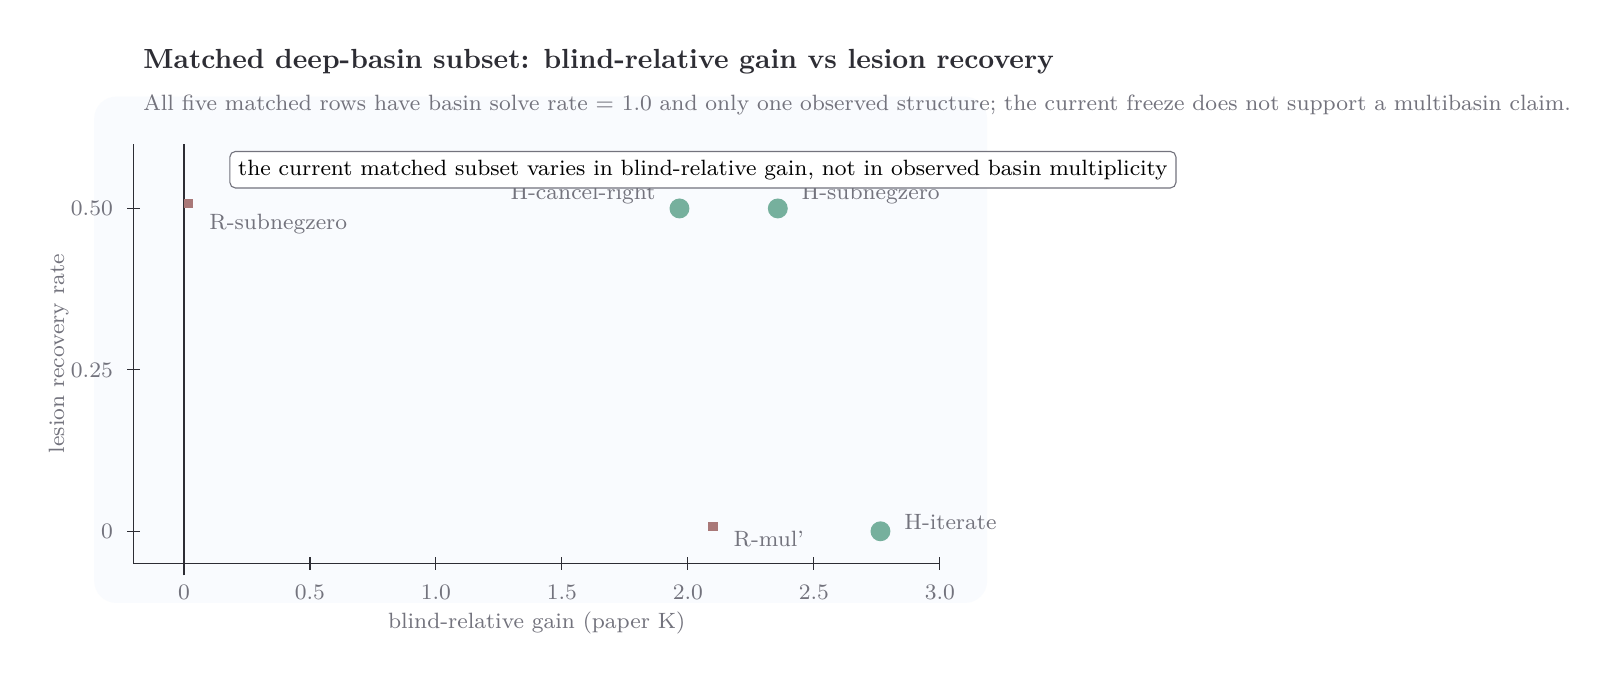
\begin{tikzpicture}[
    every node/.style={font=\small},
    show background rectangle,
    background rectangle/.style={fill=white}
]

\def\xmin{-0.2}
\def\xmax{3.0}
\def\ymin{-0.05}
\def\ymax{0.60}
\def\xscale{3.2}
\def\yscale{8.2}

\path[fill=basin1!18, rounded corners=8pt] (-0.5, -0.5) rectangle ({(\xmax-\xmin)*\xscale + 0.6}, {(\ymax-\ymin)*\yscale + 0.6});

\node[paneltitle, anchor=west] at (0, {(\ymax-\ymin)*\yscale + 1.05}) {Matched deep-basin subset: blind-relative gain vs lesion recovery};
\node[annot, anchor=west] at (0, {(\ymax-\ymin)*\yscale + 0.5}) {All five matched rows have basin solve rate = 1.0 and only one observed structure; the current freeze does not support a multibasin claim.};

\draw[ink, line width=0.6pt] (0, 0) -- ({(\xmax-\xmin)*\xscale}, 0);
\draw[ink, line width=0.6pt] ({(0-\xmin)*\xscale}, -0.15) -- ({(0-\xmin)*\xscale}, {(\ymax-\ymin)*\yscale});
\draw[ink, line width=0.6pt] (0, 0) -- (0, {(\ymax-\ymin)*\yscale});

\foreach \x/\label in {0.0/0, 0.5/0.5, 1.0/1.0, 1.5/1.5, 2.0/2.0, 2.5/2.5, 3.0/3.0} {
    \draw[ink, line width=0.4pt] ({(\x-\xmin)*\xscale}, -0.08) -- ({(\x-\xmin)*\xscale}, 0.08);
    \node[annot, anchor=north] at ({(\x-\xmin)*\xscale}, -0.14) {\label};
}
\foreach \y/\label in {0.0/0, 0.25/0.25, 0.50/0.50} {
    \draw[ink, line width=0.4pt] (-0.08, {(\y-\ymin)*\yscale}) -- (0.08, {(\y-\ymin)*\yscale});
    \node[annot, anchor=east] at (-0.14, {(\y-\ymin)*\yscale}) {\label};
}

\node[annot] at ({(\xmax-\xmin)*\xscale/2}, -0.75) {blind-relative gain (paper K)};
\node[annot, rotate=90] at (-0.95, {(\ymax-\ymin)*\yscale/2}) {lesion recovery rate};

% heuristic points
\fill[accentgreen!80] ({(2.35679-\xmin)*\xscale}, {(0.5-\ymin)*\yscale}) circle[radius=3.6pt];
\node[annot, anchor=west] at ({(2.35679-\xmin)*\xscale + 0.18}, {(0.5-\ymin)*\yscale + 0.18}) {H-subnegzero};

\fill[accentgreen!80] ({(2.764221-\xmin)*\xscale}, {(0.0-\ymin)*\yscale}) circle[radius=3.6pt];
\node[annot, anchor=west] at ({(2.764221-\xmin)*\xscale + 0.18}, {(0.0-\ymin)*\yscale + 0.12}) {H-iterate};

\fill[accentgreen!80] ({(1.966517-\xmin)*\xscale}, {(0.5-\ymin)*\yscale}) circle[radius=3.6pt];
\node[annot, anchor=east] at ({(1.966517-\xmin)*\xscale - 0.18}, {(0.5-\ymin)*\yscale + 0.18}) {H-cancel-right};

% reprover points
\fill[blocked!75] ({(0.0-\xmin)*\xscale}, {(0.5-\ymin)*\yscale}) rectangle ++(0.12,0.12);
\node[annot, anchor=west] at ({(0.0-\xmin)*\xscale + 0.20}, {(0.5-\ymin)*\yscale - 0.20}) {R-subnegzero};

\fill[blocked!75] ({(2.080518-\xmin)*\xscale}, {(0.0-\ymin)*\yscale}) rectangle ++(0.12,0.12);
\node[annot, anchor=west] at ({(2.080518-\xmin)*\xscale + 0.20}, {(0.0-\ymin)*\yscale - 0.10}) {R-mul'};

\node[formula, anchor=west] at ({(0.18-\xmin)*\xscale}, {(0.56-\ymin)*\yscale}) {the current matched subset varies in blind-relative gain, not in observed basin multiplicity};

\end{tikzpicture}
\end{document}
